\section{Hybrid Flexible Flowshop with Transportation Times}


\begin{frame}
\frametitle{Joint work with}
\begin{itemize}
\item Michele Garraffa
\item Barry O'Sullivan
\item Eddie Armstrong (J\&J Research, Limerick)
\end{itemize}
\end{frame}

\subsection{Introduction}

\begin{frame}
\frametitle{Real-World Problem}
\begin{itemize}
\item Manufacturing Industry
\item Move away from dedicated, high volume standard production
\item Allow for increasing customization of product to customer needs
\item Take advantage of more flexible, universal machines
\item Decentralize production
\end{itemize}
\end{frame}

\begin{frame}
\frametitle{Research Challenges}
\begin{itemize}
\item Consider transport time in flowshop scheduling
\item Choose appropriate technology to solve problem
\item Study realistic scenarios at scale
\end{itemize}
\end{frame}

% \begin{frame}
% \frametitle{What we will discuss}
% \begin{itemize}
% \item New variant of known scheduling problem
% \begin{itemize}
% \item Hybrid Flexible Flowshop with Transportation Times
% \item Solved with different approaches
% \begin{itemize}
% \item CP (4 Versions)
% \item MIP (5 Versions)
% \item Local Search
% \end{itemize}
% \item Spoiler: CP works well, MIP not so much
% \end{itemize}
% \item Factory layout problem
% \begin{itemize}
% \item How does the layout affect the scheduling?
% \item Compare different high level design scenarios
% \end{itemize}
% \end{itemize}
% \end{frame}

\begin{frame}
\frametitle{A bit of Background}
\begin{textblock*}{4cm}(11cm,2cm)

\includegraphics[width=4cm]{imagesjj/1000px-Johnson_and_Johnson_Logo.png}
\end{textblock*}
\begin{textblock*}{4cm}(11cm,4cm)

\includegraphics[width=4cm]{imagesjj/confirm.png}
\end{textblock*}
\begin{itemize}
\item Johnson\&Johnson is a large multi-national company
\begin{itemize}
\item Strong production and research presence in Ireland
\item Focus on consumer health, medical devices, pharmaceuticals
\end{itemize}
\item Confirm
\begin{itemize}
\item Irish National SFI Centre focussed on Manufacturing
\item Includes groups from multiple universities
\item Our focus is on analytics/optimization
\item Complements our work in the Insight SFI Centre for Data Analytics
\end{itemize}
\end{itemize}
\end{frame}

\subsection{Problem Description}

\begin{frame}
\frametitle{Flexible Factory Structure (Including Transport Between Machines)}
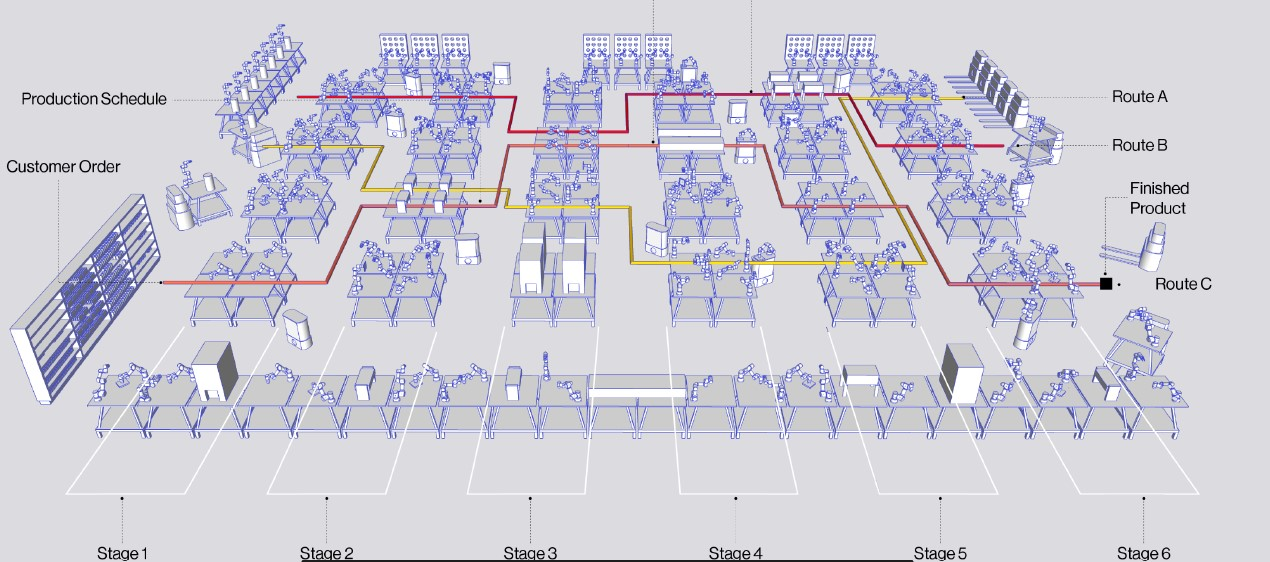
\includegraphics[width=14cm]{imagesjj/factory}
\end{frame}

\begin{frame}
\frametitle{Main Elements of Problem}
\begin{itemize}
\item Flow shop
\begin{itemize}
\item Jobs run through production in the same sequence
\end{itemize}

\item Hybrid
\begin{itemize}
\item Multiple, identical machines available in each stage
\end{itemize}

\item Flexible
\begin{itemize}
\item Some production stages may be skipped for certain jobs
\end{itemize}

\item Transportation Time
\begin{itemize}
\item Time for transport between stage is significant, but not a resource limit
\item Many robots to handle transport tasks
\item Typical machine layout in lanes
\end{itemize}

\item Objective makespan
\begin{itemize}
\item Production not driven by due dates
\end{itemize}
\end{itemize}
\end{frame}

% \begin{frame}
% \frametitle{Why is this interesting?}
% \begin{itemize}
% \item Industrial Use Case

% \item Increased complexity over existing hybrid flexible flowshop

% \item Machines in each stage are no longer exchangeable in schedule
% \begin{itemize}
% \item Reduced symmetry
% \item But also preferred paths through factory
% \end{itemize}

% \end{itemize}
% \end{frame}

% \begin{frame}
% \frametitle{Not Considered in this Study}
% \begin{itemize}
% \item Sequence dependent setup times
% \begin{itemize}
% \item Machines are highly flexible, do not require setup times
% \end{itemize}

% \item Buffer space
% \begin{itemize}
% \item Manufactured items are quite small
% \item Trays can be stacked in front of machines
% \end{itemize}

% \item Different production speed on machines of same stage
% \begin{itemize}
% \item Assumes same generation of machines within each stage
% \item (Different stages have different processing
% \end{itemize}

% \item Resource limits on transport
% \begin{itemize}
% \item No congestion in transport lanes
% \item Enough robots to keep material flowing through plant
% \end{itemize}
% \end{itemize}
% \end{frame}

\begin{frame}
\frametitle{Objectives of Project}
\begin{itemize}
\item Identify best tools to schedule new plant
\begin{itemize}
\item Explore variety of different approaches and techniques
\item Do not just focus on your preferred solution method/solver
\end{itemize}

\item Answer some design questions before committing to one approach
\begin{itemize}
\item Is it better to have one or multiple facilities?
\item How far should the transport reach between lanes?
\item How can we exploit flexibility in new machines to offer better products?
\begin{itemize}
\item Semi custom production
\end{itemize}
\end{itemize}

\item Provide some quantitative comparison based on typical production data
\begin{itemize}
\item Not currently for operational scheduling
\end{itemize}

\end{itemize}
\end{frame}

\subsection{Models}

\begin{frame}
\frametitle{CP Models}
\begin{itemize}
\item Two main modelling alternatives
\begin{itemize}
\item Diffn model to handle machine choice
\item Interval Task Variables with optional tasks on all alternative machines
\end{itemize}

\item Transportation time handled by table constraint
\begin{itemize}
\item Transportation between machines for tasks of the same job
\item Much simpler case than sequence dependent setup
\end{itemize}

\item Precedences between tasks of jobs

\item Objective Cmax makespan

\end{itemize}
\end{frame}

\begin{frame}
\frametitle{CP Model Main Alternative}
\begin{tabular}{cc}
\scalebox{0.5}{
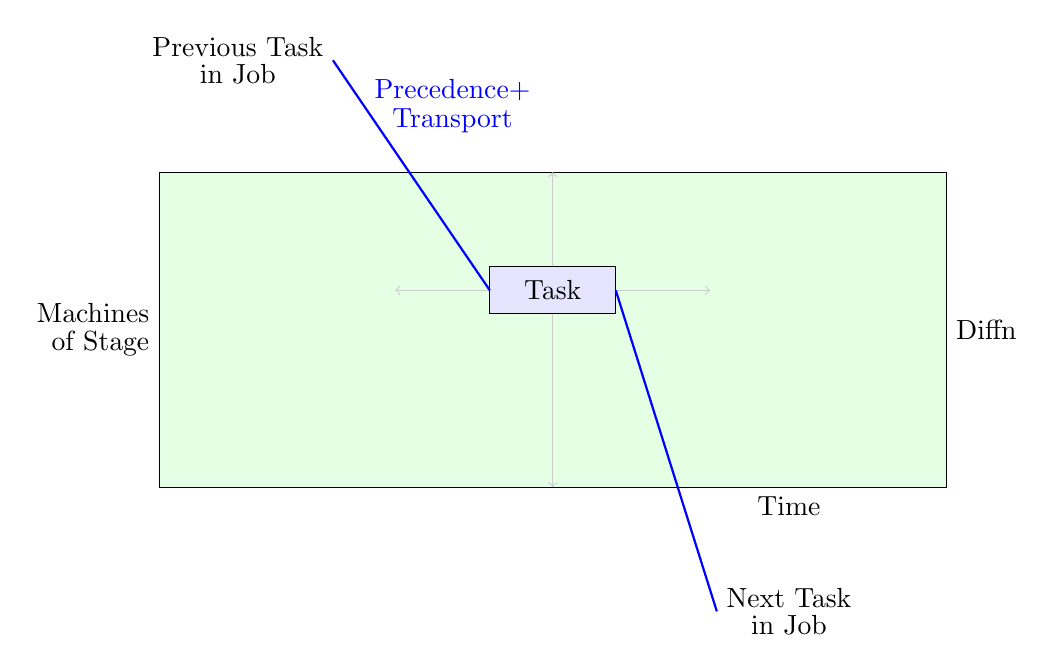
\begin{tikzpicture}
  \draw[draw=black,fill=green!10] (0,0) rectangle (10,4);
  \node[right] () at (10,2.0) {Diffn};
  \draw[black!20,<->] (3,2.5) -- (7,2.5);
  \draw[black!20,<->] (5,0) -- (5,4);
  \draw[fill=blue!10] (4.2,2.2) rectangle node {Task} (5.8,2.8);
  \node[below] (time) at (8,0) {Time};
  \node[left] (machine) at (0,2) {\shortstack[r]{Machines\\of Stage}};
  \node[above] (prev) at (1,5) {\shortstack{Previous Task\\in Job}};
  \node[above] (next) at (8,-2) {\shortstack{Next Task\\in Job}};
  \draw[thick,blue] (prev.east) -- node[pos=0.2,right] {\shortstack{Precedence+\\Transport}} (4.2,2.5);
  \draw[thick,blue] (next.west) -- (5.8,2.5);
\end{tikzpicture}
}
&
\scalebox{0.5}{
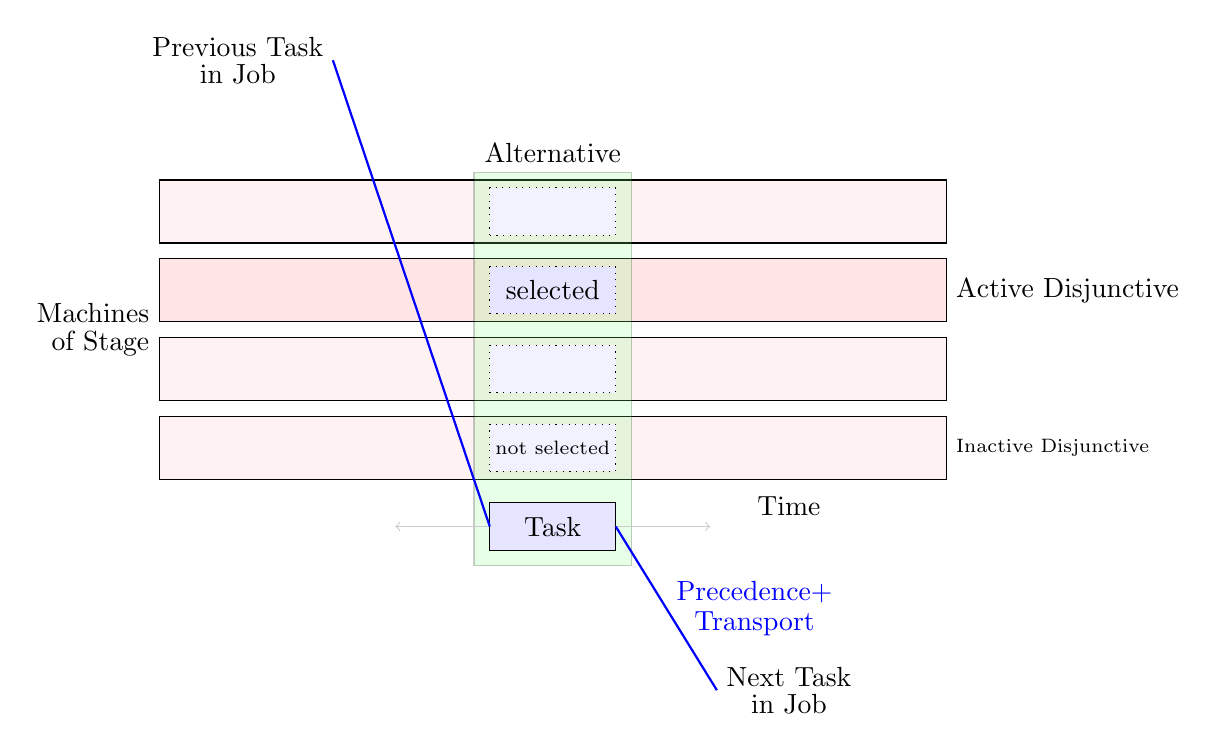
\begin{tikzpicture}
  \draw[draw=black,fill=red!5] (0,0.1) rectangle (10,0.9);
  \draw[draw=black,fill=red!5] (0,1.1) rectangle (10,1.9);
  \draw[draw=black,fill=red!10] (0,2.1) rectangle (10,2.9);
  \draw[draw=black,fill=red!5] (0,3.1) rectangle (10,3.9);
  \node[right] () at (10,2.5) {Active Disjunctive};
  \node[right] () at (10,0.5) {\scriptsize Inactive Disjunctive};
  \draw[fill=green!50,opacity=0.2] (4,-1) rectangle (6,4);
  \node[above] () at (5,4) {Alternative};
  \draw[dotted,fill=blue!5] (4.2,0.2) rectangle node {\scriptsize not selected} (5.8,0.8);
  \draw[dotted,fill=blue!5] (4.2,1.2) rectangle (5.8,1.8);
  \draw[dotted,fill=blue!10] (4.2,2.2) rectangle node {selected} (5.8,2.8);
  \draw[dotted,fill=blue!5] (4.2,3.2) rectangle (5.8,3.8);
  \draw[black!20,<->] (3,-0.5) -- (7,-0.5);
  \draw[fill=blue!10] (4.2,-0.2) rectangle node {Task} (5.8,-0.8);
  \node[below] (time) at (8,0) {Time};
  \node[left] (machine) at (0,2) {\shortstack[r]{Machines\\of Stage}};
  \node[above] (prev) at (1,5) {\shortstack{Previous Task\\in Job}};
  \node[above] (next) at (8,-3) {\shortstack{Next Task\\in Job}};
  \draw[thick,blue] (prev.east) -- (4.2,-0.5);
  \draw[thick,blue] (next.west) -- node[right] {\shortstack{Precedence+\\Transport}} (5.8,-0.5);
\end{tikzpicture}
}
\end{tabular}

\end{frame}

\begin{frame}
\frametitle{Dedicated MIP Models}
\begin{itemize}
\item Four alternatives based on literature for hybrid flexible flowshop
\item Adding transportation time grows model complexity
\item Picked best alternative on small scale test cases
\item None of the methods scale to expected problem sizes
\end{itemize}
\end{frame}

\begin{frame}
\frametitle{Dispatch Rule/Local Search}
\begin{itemize}
\item To provide baseline result/ initial upper bound

\item Schedule jobs in random order

\item Assign each task to first available machine

\item Dispatch Rule
\begin{itemize}
\item Explore different initial job permutations
\end{itemize}

\item Local Search
\begin{itemize}
\item Also explore swaps/insertion of jobs in sequence
\end{itemize}

\item Written in Java
\end{itemize}
\end{frame}

\begin{frame}
\frametitle{Implementations}
\begin{itemize}
\item MiniZinc, Chuffed, free search
\begin{itemize}
\item Diffn constraint
\end{itemize}

\item MiniZinc, Chuffed, priority search

\item MiniZinc (interval task variables)

\item MiniZinc, Cplex

\item MIP model, Cplex

\item CP Optimizer (interval task variables, black box search)

\item SICStus Prolog diffn model, custom search)
\end{itemize}
\end{frame}

\subsection{First Experiment: Compare different solution methods}

\begin{frame}
\frametitle{Instance Generator}
\begin{itemize}
\item Produce sequence of test cases with increasing number of jobs
\begin{itemize}
\item 20, 25, 30, 40, 50, 100, 200, 300, 400 jobs
\item 25 instances per problem size
\end{itemize}

\item Parameters chosen to reflect real world factory
\begin{itemize}
\item 8 stages, 10 machines/stage, some skipped stages
\item Discrete power law for job types
\begin{itemize}
\item A few products are quite common, many are rare in order set
\end{itemize}
\item Transport times based on lanes
\end{itemize}

\item Instances available on line
\begin{itemize}
\item \url{https://zenodo.org/record/5168966}
\end{itemize}

\end{itemize}
\end{frame}

\begin{frame}
\frametitle{Experimental Setup}
\begin{itemize}
\item Experiments run on single core of Windows 10 laptop

\item Timeout 300s

\item Upper bound provided by 10s of Local Search

\item Best lower bound provided to stop search for optimal solutions
\begin{itemize}
\item Optimal solutions found for many smaller (20 30 jobs) instances
\end{itemize}

\end{itemize}
\end{frame}

\begin{frame}
\frametitle{Cmax Results with Different Models (average over 25 instances, 300s timeout)}
\begin{tabular}{*{10}{r}}\toprule
Size & \shortstack{Lower\\Bound} & \shortstack{Upper\\Bound}& \shortstack{CP\\Opt}& \shortstack{Chuffed\\Free}& \shortstack{Chuffed\\Priority}& \shortstack{Dispatch\\Rule}& \shortstack{Local\\Search}& SICStus\\ \midrule
20 & 61.88 & 63.56& \ccg 62.72& 63.48& 63.04& 63.28& 63.20& \ccg 62.72\\
25 & 62.84 & 65.96& 64.24& -& 64.76& 65.20& 64.84& \ccg 64.16\\
30 & 64.12 & 70.24& \ccg 66.68& -& 68.44& 69.16& 68.24& 66.84\\
40 & 65.32 & 77.36& \ccg 72.56& -& 75.40& 76.08& 75.28& 73.28\\
50 & 67.24 & 84.52& \ccg 78.40& -& 82.24& 83.16& 82.24& 79.40\\
100 & 94.72 & 120.12& 115.16& -& 116.96& 118.28& 118.92& \ccg 113.04\\
200 & 153.08 & 185.16& 180.48& -& 181.32& 182.80& 184.76& \ccg 176.72\\
300 & 214.96 & 249.12& 248.96& -& 248.76& 246.96& 248.88& \ccg 240.96\\
400 & 275.36 & 311.60& 311.28& -& -& 308.76& 311.40& \ccg 303.16\\
\bottomrule
\end{tabular}

\end{frame}

\begin{frame}
\frametitle{Comments}
\begin{itemize}
\item CP Optimizer and SICStus perform best
\begin{itemize}
\item CP Optimizer better for small/medium instances
\item SICStus does scale better
\item Note: SICStus uses hand made search routine
\item Chuffed free search does not scale at all
\begin{itemize}
\item Very poor improvements on makespan
\end{itemize}
\item Chuffed priority search: good initial solutions only
\end{itemize}

\item Dispatch Rule and Local Search perform quite well
\begin{itemize}
\item Further development potential
\end{itemize}

\item MIP does not work at all
\begin{itemize}
\item Limited to smaller instances not shown here
\end{itemize}

\end{itemize}
\end{frame}

\subsection{Second Experiment: Study layout alternatives}

\begin{frame}
\frametitle{Four Layout Alternatives (One or Two Locations)}
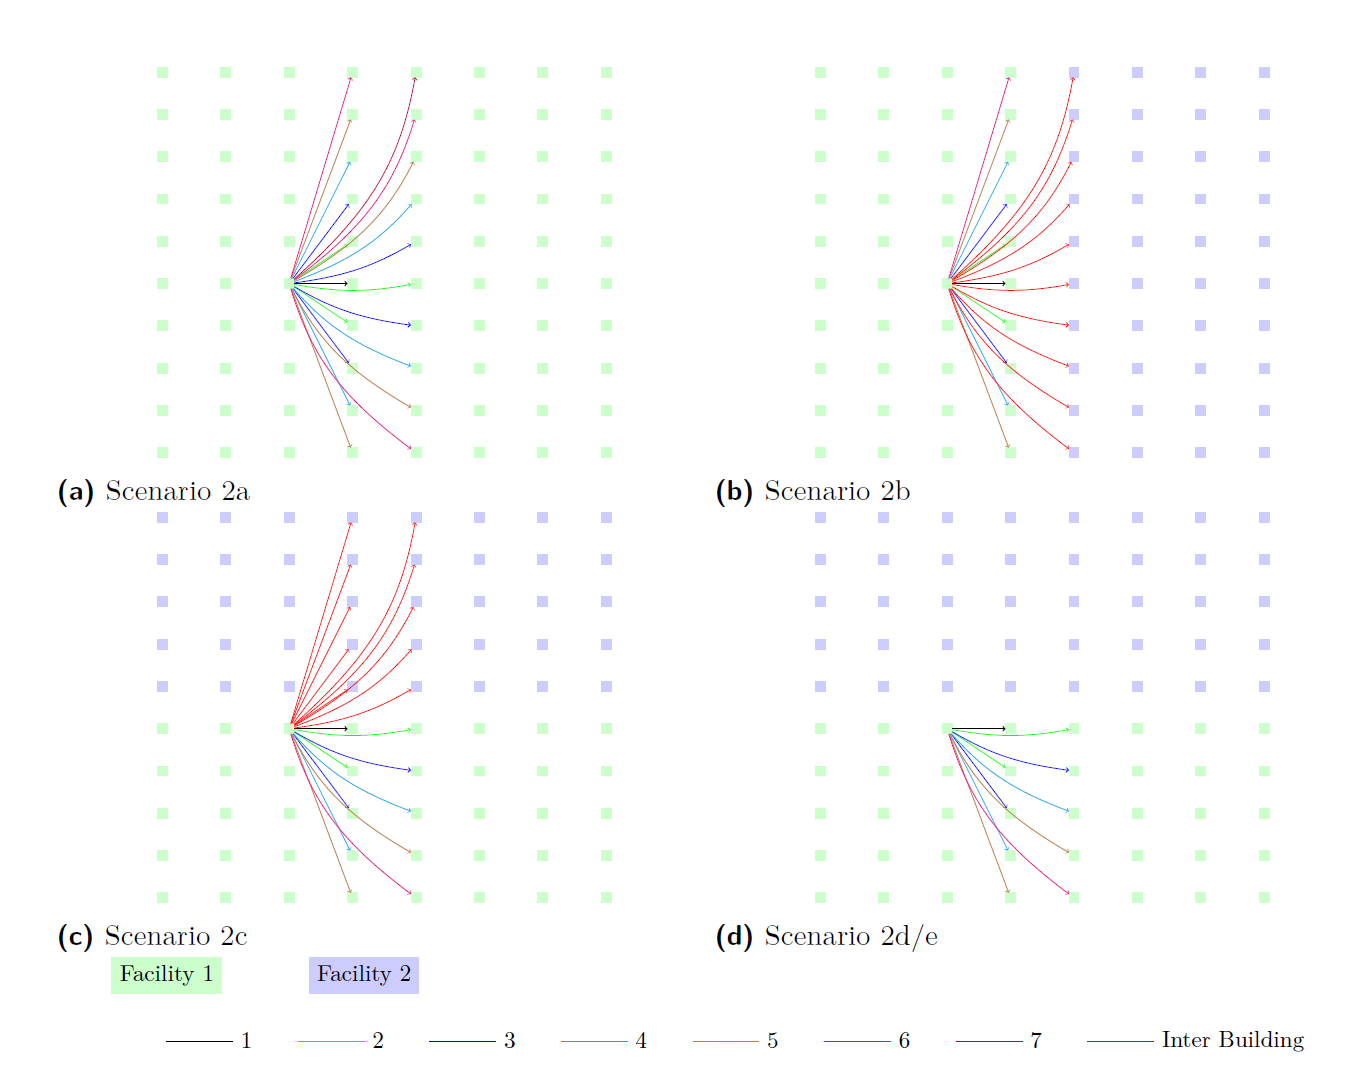
\includegraphics[width=8.8cm]{imagesjj/layoutalternatives}
\end{frame}


\begin{frame}
\frametitle{Five Scenarios Tested}
\begin{description}
\item[2a] Single facility organized in lanes

\item[2b] Two facilities in sequence (sequential for all jobs)

\item[2c] Two facilities in parallel with transport between facilities allowed

\item[2d] Two facilities in parallel, transport only within each facility

\item[2e] Two factories in parallel, with 80\% of jobs preassigned to a factory

\end{description}
\end{frame}

\begin{frame}
\frametitle{Scenario Comparison}
\begin{tabular}{l*{7}{r}}\toprule
       &   & \multicolumn{5}{c}{Scenario} & \\
Solver & Size  & 2a & 2b & 2c & 2d & 2e \\ \midrule
SICStus & 200  & \ccg 176.84& \ccg 184.84& \ccg 178.28& \ccg 180.52& \ccg 180.48 \\
\multicolumn{2}{l}{\% over Best}    &  0.00&  4.52&  0.81&  2.08\\
CPOptimizer & 200 & 184.40& 190.92& 186.00& 183.52& 183.52\\
\multicolumn{2}{l}{\% over Best}&  1.23&  4.81&  2.11&  0.75\\
Dispatch &200  & 182.76& 190.44& 184.28& 184.60& 184.64 \\
\multicolumn{2}{l}{\% over Best}&  0.00&  4.20&  0.83&  1.01\\
Local Search &200 & 184.68& 192.24& 185.76& 186.08& 185.96\\
\multicolumn{2}{l}{\% over Best}&  0.13&  4.23&  0.72&  0.89\\
\bottomrule
\end{tabular}

\end{frame}

\subsection{Summary}

\begin{frame}
\frametitle{Summary}
\begin{itemize}
\item New variant of known scheduling problem
\begin{itemize}
\item Arising from flexible new factory design

\item Transportation between machines/locations important element of schedule

\item Good solutions are obtained with CP for large problem instances

\item Not all CP models achieve the same solution quality
\item MIP results weak
\item Remaining, open gap between best lower bound and best solution found
\end{itemize}

\item Scheduling model used for factory design study
\begin{itemize}
\item Which layout gives the best overall results?
\item Explores four design alternatives
\end{itemize}

\end{itemize}
\end{frame}


\begin{frame}
\frametitle{Results Scale to Hundreds of Jobs (shown: SICStus 1000 jobs, 80 machines)}
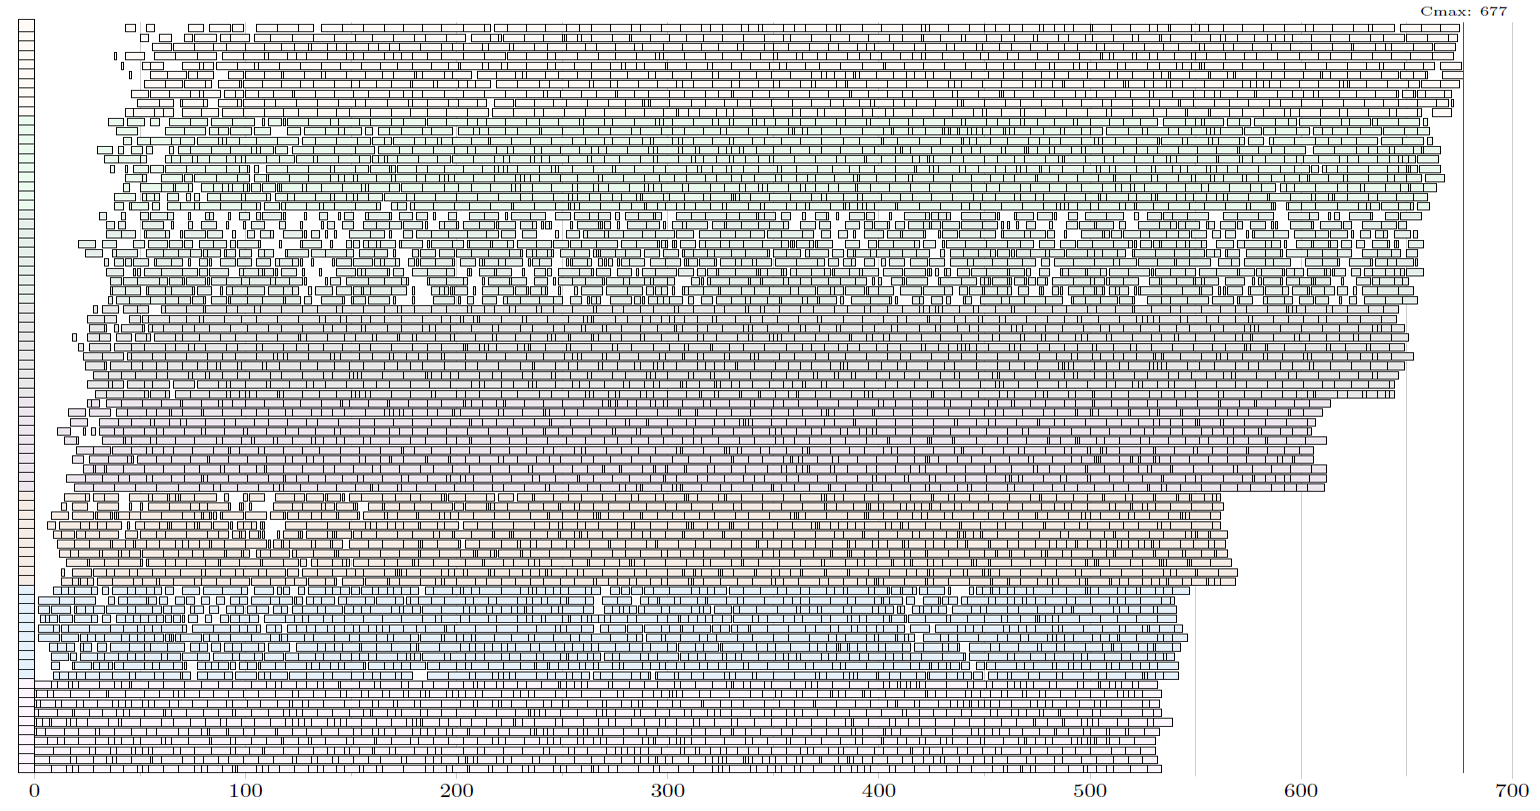
\includegraphics[width=14cm]{imagesjj/ganttchart}
\end{frame}







